\documentclass[a4paper,12pt]{article}
%%%%%%%%%%%%%%%%%%%%%%%%%%%%%%%%%%%%%%%%%%%%%%%%%%%%%%%%%%%%%%%%%%%%%%%%%%%%%%%%%%%%%%%%%%%%%%%%%%%%%%%%%%%%%%%%%%%%%%%%%%%%%%%%%%%%%%%%%%%%%%%%%%%%%%%%%%%%%%%%%%%%%%%%%%%%%%%%%%%%%%%%%%%%%%%%%%%%%%%%%%%%%%%%%%%%%%%%%%%%%%%%%%%%%%%%%%%%%%%%%%%%%%%%%%%%
\usepackage{eurosym}
\usepackage{vmargin}
\usepackage{amsmath}
\usepackage{graphics}
\usepackage{epsfig}
\usepackage{subfigure}
\usepackage{fancyhdr}
\usepackage{listings}
\usepackage{framed}
\usepackage{graphicx}
\usepackage{amsmath}
\usepackage{chngpage}
%\usepackage{bigints}


\setcounter{MaxMatrixCols}{10}

\begin{document}
	\large
%%- http://dev.socrata.com/consumers/examples/data-visualization-with-python.html

%==================================%


\begin{figure}[h!]
\centering
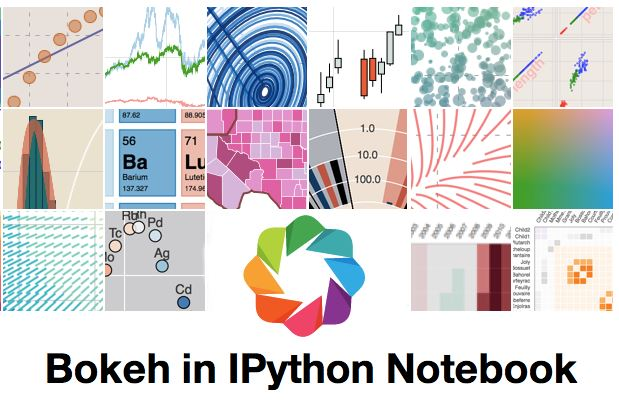
\includegraphics[width=0.9\linewidth]{images/TitleSlide}
\end{figure}

\begin{quote}
Bokeh is a Python interactive visualization library for large datasets that natively uses the latest web technologies. Its goal is to provide elegant, concise construction of novel 
graphics in the style of Protovis/D3, while delivering high-performance interactivity over large data to thin clients.

\end{quote}
\newpage
\begin{itemize}
\item Bokeh is developed by \textbf{Continuum Analytics}.
\end{itemize}
\begin{figure}[h!]
\centering
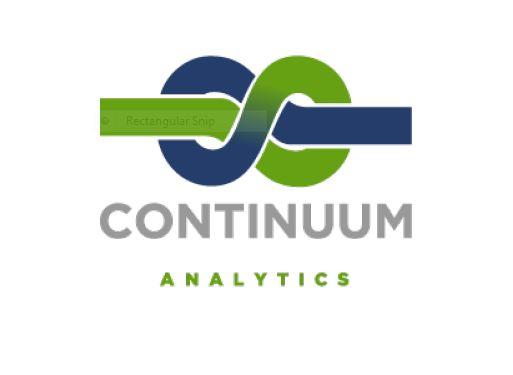
\includegraphics[width=1.0\linewidth]{images/continuum}
\end{figure}

\begin{figure}[h!]
\centering
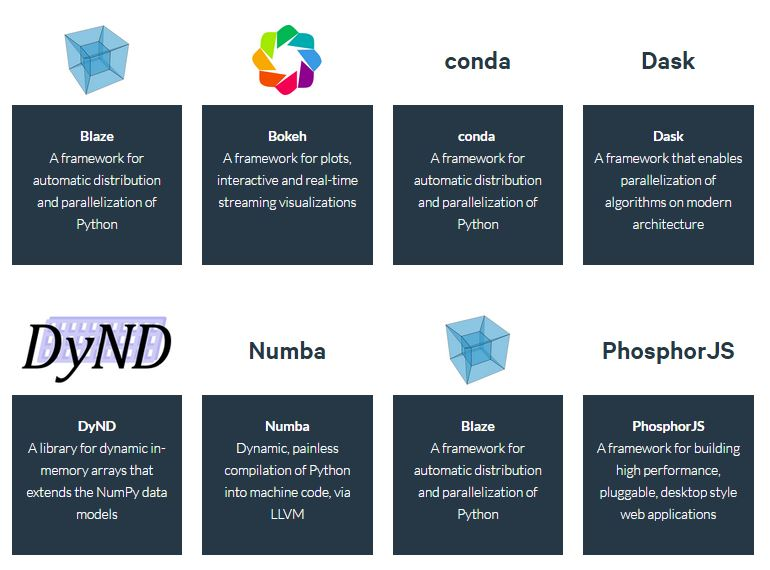
\includegraphics[width=0.9\linewidth]{images/00-continuum-projects}
\end{figure}
\newpage
\section*{Bokeh scales visualization to Big Data}
\textit{(From Bokeh Documentation)}
\begin{itemize}
\item Interactive and real-time streaming visualization framework that scales to Big Data with data shading

\item Bokeh is a Python data visualization library combining the ideas of the \textbf{Grammar of Graphics} and \textbf{Protovis}, with enhancements to support interactive visualization. Its primary output backend is HTML5 Canvas.

\item There are many excellent plotting packages for Python, but they generally do not optimize for the particular needs of statistical plotting or multidimensional datasets. 
\item Additionally, advanced visual customization is typically difficult for non-programmers, and most libraries do not build a reified data processing pipeline that supports rich interactivity like linked brushing. 
\item Bokeh addresses these problems at their core by using a declarative data transformation scheme, and is engineered to operate in a client/server model for the modern web.


\item Bokeh can produce elegant and interactive visualization like D3.js with high-performance interactivity over very large or streaming datasets. Bokeh can help anyone who would like to quickly and easily create interactive plots, dashboards, and data applications.
\end{itemize}

\newpage
%==================================%
\begin{framed}
	\noindent \textbf{Benefits of Bokeh:}
	
	\begin{itemize}
		\item Bokeh allows you to build complex statistical plots quickly and through simple commands
		\item Bokeh provides you output in various medium like html, notebook and server
		\item We can also embed Bokeh visualization to flask and django app
		\item Bokeh can transform visualization written in other libraries like matplotlib, seaborn, ggplot
		\item Bokeh has flexibility for applying interaction, layouts and different styling option to visualization
	\end{itemize}
\end{framed}
%==================================%
\newpage
\subsection*{Installation}
You may need to install a few Python packages :


\begin{framed}
\begin{verbatim}
conda install pandas
conda install bokeh
\end{verbatim}
\end{framed}

\subsection*{IMPORTANT : Version}

\begin{figure}[h!]
\centering
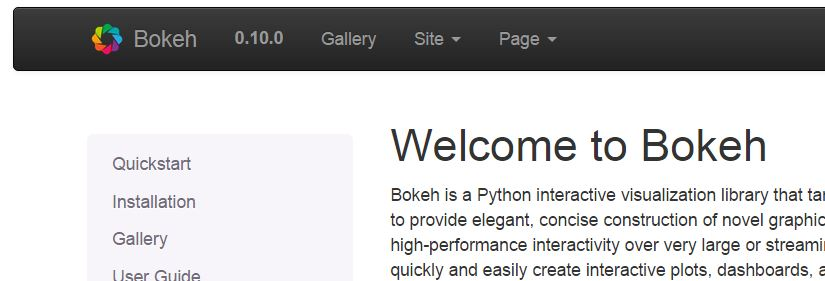
\includegraphics[width=0.7\linewidth]{images/00-BOKEH-version}
\end{figure}
\begin{itemize}
\item This workshop will be based on version 0.10. 
\item A lot of code for older version of Bokeh no longer work.
\item To check what version you actually have installed, run the following code
\end{itemize}


\begin{figure}[h!]
	\centering
	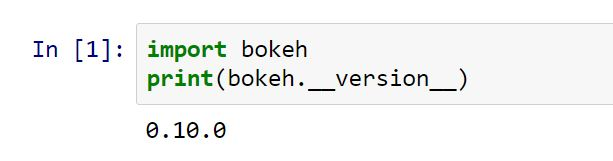
\includegraphics[width=0.9\linewidth]{images/00-BOKEH-version-check}
\end{figure}
%==================================%
\newpage
\begin{framed}
	\noindent \textbf{Challenges with Bokeh}
	\begin{itemize}
		\item Like with any upcoming open source library, Bokeh is undergoing a lot of development. So, the code you write today may not be entirely reusable in future.
		
		\item  It has relatively less visualization options, when compared to \textbf{\textit{D3.js}}. Hence, it is unlikely in near future that it will challenge \textbf{\textit{D3.js}} for its crown.
		\item  Given the benefits and the challenges, it is currently ideal to rapidly develop prototypes. However, if you want to create something for production environment, \textbf{\textit{D3.js}} might still be your best bet.
	\end{itemize}
\end{framed}
%==================================%
\newpage


%==================================%
\end{document}

Introduction

Recently, I was going through a video from SciPy 2015 conference, “Building Python Data Apps with Blaze and Bokeh“, recently held at Austin, Texas, USA. I couldn’t stop thinking about the power these two libraries provide to data scientists using Python across the globe. In this article, I will introduce you to the world of possibilities in data visualization using Bokeh and why I think this is a must learn / use library for every data scientist out there.

Bokeh_Introduction Source: bokeh.pydata.org


\noindent \textbf{What is Bokeh?}

Bokeh is a Python library for interactive visualization that targets web browsers for representation. This is the core difference between Bokeh and other visualization libraries. Look at the snapshot below, which explains the process flow of how Bokeh helps to present data to a web browser.

Bokeh_IntroSource: Continuum Analytics


As you can see, Bokeh has multiple language bindings (Python, R, lua and Julia). These bindings produce a JSON file, which works as an input for BokehJS (a Javascript library), which in turn presents data to the modern web browsers.


\end{frame}
%==================================%
%==================================%
\begin{frame} 

What does Bokeh offer to a data scientist like me?

I started my data science journey as a BI professional and then worked my way through predictive modeling, data science and machine learning. I have primarily relied on tools like QlikView & Tableau for data visualization and SAS & Python for predictive analytics & data science. I had near zero experience of using JavaScript.

So, for all my data products or ideas, I had to either outsource the work or had to pitch my ideas through wire-frames, both of which are not ideal for building quick prototypes. Now, with Bokeh, I can continue to work in Python ecosystem, but still create these prototypes quickly.
\end{frame}
%==================================%


%==================================%
\begin{frame}
\framtitle{Installing Bokeh}
To install Bokeh, please follow the instruction given here.


%========================================================================%

Getting Set Up
Install Bokeh and verify your installation is working correctly.
Defining Key Concepts
Define and explain important preliminary concepts.
Plotting with Basic Glyphs
Use the simple but flexible glyph methods from the bokeh.plotting interface to construct basic and custom plots.

Using High-level Charts
Use the high-level bokeh.charts interface to create common statistical charts quickly and easily.
Leveraging Other Libraries
Display a wide range of plots created using Matplotlib, Seaborn, pandas, or ggplot.py as Bokeh plots.
Styling Visual Attributes
Customize every visual aspect of Bokeh plots—axes, grids, labels, glyphs, and more.
Configuring Plot Tools
Make interactive tools (like pan, zoom, select, and others) available on your plots.

Laying Out Multiple Plots
Combine multiple plots and widgets into specified layouts.
Working in the Notebook
Creating and display interactive plots inside Jupyter/IPython notebooks.

Adding Interactions
Create more sophisticated interactions including widgets or linked panning and selection.
Deploying the Bokeh Server
Deploy the Bokeh Server to build and publish sophisticated data applications.
Embedding Bokeh Plots
Embed static or server-based Bokeh plots and widgets into HTML documents in a variety of ways.
Speeding up visualizations with WebGL
Improve performance for large datasets by using WebGL.

%================================================================ %